\vspace{-.2em}
\section{Main Method}\label{sec:main_method}
\vspace{-.2em}
In this section, we first introduce two objectives for reward-function learning
based on the classical approaches in the learning-to-rank (LTR) literature \citep{liu2009learning}.
Then we use MinTL \citep{mintl2020} as an example to demonstrate how we can use the learned reward function as a plugin module to improve existing methods of training the E2E ToD models.

% \subsection{Overview of the Training Process}\label{sec:method_overview}
% \st{TODO: @yihao describe the training process, how we get multiple alternative dialogue trajectories, and how to rank them (call the score s)}
\vspace{-.4em}
\subsection{Two Generalized Objectives for Reward Learning}\label{sec:main_rew_obj}
\vspace{-.4em}
%Instead of learning the reward function $\gR_{\theta}(o_t, a_t, g)$ via the pairwise preference learning, 
We introduce two objectives, \texttt{RewardNet} and \texttt{RewardMLE}, both of which can utilize multiple dialogue trajectories 
on each update for optimizing the reward function.
Our motivation is that, compared with the pairwise approach described in Eq.~\eqref{eq:original_pref_rew}, these two objectives consider more information at each training step, and thus can be more effective for reward learning and may lead to a better solution under the stochastic training setting.
% , these two objectives can improve efficiency of the reward learning, especially under the stochastic training settings.

\myparagraph{Setup.}
Assume that there are $N \geq 2$ dialogue trajectories, denoted by $\gD_{N} \triangleq (\tau_1, \tau_2, \ldots, \tau_N)$, 
and each trajectory $\tau_i$ has an automatic evaluation score $S(\tau_i)$.\footnote{We use the \texttt{Combined Score} \citep{sfnrl2019} as $S(\tau_i)$. Detailed definition is delayed to \Secref{sec:exp}.}
For simplicity, we assume that these $N$ dialogue trajectories are of equal length $T$ and are already sorted by the automatic evaluation scores, \ie, $ \tau_1 \succ \tau_2 \succ \cdots \succ \tau_N$, or equivalently, $S(\tau_1) > S(\tau_2) > \cdots > S(\tau_N)$.
We denote the accumulated reward of dialogue trajectory $\tau_i$ from $\gR_\theta$ as $J(\tau_i; \theta)= \sum_{t=0}^{T}\gR_{\theta}(o_t^{(i)},a_t^{(i)}, g^{(i)})$.
Our goal is to learn a reward function $\gR_{\theta}(o, a, g)$ such that the accumulated rewards of those trajectories can reflect the ranking order, \ie, 
$J(\tau_1; \theta) > \cdots > J(\tau_N; \theta)$. 

\myparagraph{\texttt{RewardNet}.}
The proposed \texttt{RewardNet} objective for reward function learning is adapted from the \textit{ListNet} loss \citep{listnet2007} in the LTR literature. 
Specifically, given $N$ trajectories and their associated scores, we 
define the \texttt{RewardNet} loss as the cross entropy between $\{J(\tau_i; \theta)\}_{i=1}^{N}$ and $\{S(\tau_i)\}_{i=1}^{N}$:
% \begin{align}\textstyle
%     \ell_{\texttt{RewardNet}}(\theta; \gD_{N} ) \triangleq& - \sum_{i=1}^{N} P_{S}(\tau_i)\cdot \log\left( P_{J(\tau ; \theta)}(\tau_i)\right)\,, \label{eq:listnet}\\ 
%     \text{with} ~~~~~ P_{S}(\tau_i) = {S(\tau_i)} \bigg/ {\sum_{k=1}^{N} S(\tau_k)} ,&~~~~ P_{J(\tau ; \theta)}(\tau_i) = \Phi(J(\tau_i; \theta)) \bigg/ \sum_{k=1}^{N}\Phi(J(\tau_k; \theta)) \,, \notag 
% \end{align}
\begin{equation}\label{eq:listnet}\textstyle
\resizebox{.53\linewidth}{!}{%
$
   \ell_{\texttt{RewardNet}}(\theta; \gD_{N} ) \triangleq - \sum_{i=1}^{N} P_{S}(\tau_i)\cdot \log\left( P_{J(\tau ; \theta)}(\tau_i)\right)\,,
    $%    
}
\end{equation}
\text{with}
\begin{equation*}
\resizebox{.82\linewidth}{!}{%
$
   P_{S}(\tau_i) = {S(\tau_i)} \big/ \big({\sum_{k=1}^{N} S(\tau_k)}\big),~~~~ P_{J(\tau ; \theta)}(\tau_i) = {\Phi(J(\tau_i; \theta))}\big/ \big(\sum_{k=1}^{N}\Phi(J(\tau_k; \theta))\big)\,,
    $%    
}
\end{equation*}
where $\Phi(\cdot)$ is a monotonic positive function defined on $\mathbb{R}^{+}$, 
%which can be either identity or exponential functions.
and $P_{S}(\tau_i)$ is a normalized probability vector defined by the true evaluation scores of those $N$ trajectories. 
%\yy{ normalized  probability of dialogue trajectory $\tau_i$ (not sure?)}\st{normalized prob. defined by the true score of each trajectory, similar to Eq. 5 of the CASPI paper.}.  
Note that when $N=2$ and $\Phi$ is the identity function, \rewardnet can be viewed as a \textit{soft} version of the pairwise preference loss defined in Eq.~\eqref{eq:original_pref_rew}, where the hard binary preference labels are replaced by $\{P_{S}(\tau_i)\}_{i=1}^{N}$. 
This soft pairwise loss is adopted for reward learning in the recent CASPI paper \citep{caspi2021}.
%Besides, this special pairwise loss is also utilized in CASPI \citep{caspi2021}.
%Note that the pairwise loss proposed in CASPI \citep{caspi2021} can be viewed as a special case of \texttt{RewardNet} loss where the number of trajectories $N=2$ \st{and when $\Phi$ is the identity function}.


\myparagraph{\texttt{RewardMLE}.}
The \texttt{RewardMLE} objective is based on the \textit{ListMLE} loss \citep{listmle2008}, 
where we only utilize the ranking order in the batched dialogue trajectories $\gD_{N} $, rather than the original metric scores $\{S(\tau_i)\}_{i=1}^{N}$. 
Let $y = \mathrm{rank}(S)$ be the random variable that represents the ranking order of the dialogue trajectories ($y(\tau_i) = i, \forall\, i$, if the batched trajectories $\gD_{N}$ are sorted). 
The \texttt{RewardMLE} objective is defined as the negative log-likelihood of the ranking order $y$ under the Plackett-Luce choice model \citep{plackett1975analysis,luce2012individual} induced by the accumulated reward of each trajectory $\{J(\tau_i; \theta) \}_{i=1}^N$.
Specifically, the loss is defined as
% \begin{align}
%     \ell_{\texttt{RewardMLE}}(\theta; \gD_{N}) &\triangleq -\log P\br{y \given \{J(\tau_i; \theta)\}_{i=1}^{N}}\,, \label{eq:listmle}\\
%     \text{with}~~~~~~ P\br{y\given \{J(\tau_i; \theta)\}_{i=1}^{N}} &= \prod_{\textcolor{blue}{i=1}}^{N} \cbr{\Phi(J(\tau_i; \theta)) \bigg/ \sum_{\textcolor{blue}{k=i}}^{N}\Phi(J(\tau_k ; \theta))} \,, \notag 
% \end{align}
\begin{equation}\label{eq:listmle}\textstyle
\resizebox{.5\linewidth}{!}{%
$
  \ell_{\texttt{RewardMLE}}(\theta; \gD_{N}) \triangleq -\log P\br{y \given \{J(\tau_i; \theta)\}_{i=1}^{N}}\,,
    $%    
}
\end{equation}
with
\begin{equation*}
\resizebox{.61\linewidth}{!}{%
$
   ~~~~~~ P\br{y\given \{J(\tau_i; \theta)\}_{i=1}^{N}} = \prod_{\textcolor{blue}{i=1}}^{N} \cbr{\Phi(J(\tau_i; \theta)) \big/ \sum_{\textcolor{blue}{k=i}}^{N}\Phi(J(\tau_k ; \theta))} \,,
    $%    
}
\end{equation*}
where trajectories in $\gD_{N}$ are assumed sorted as described in the problem setup, \ie, $\tau_1 \succ \cdots \succ \tau_N$. 
Since \texttt{RewardMLE} only requires the ranking information derived from the raw scores,
it is potentially a more robust choice when the preference scores could be inaccurate.
%the ranking orders of the preference scores are favored.
%\st{
%\texttt{RewardMLE} only uses the ranking information derived from the raw scores, rather than the numerical scores themselves, it is potentially more robust than %\texttt{RewardNet} to the small inaccuracies in the raw scores.
%Such inaccuracies may be inevitable since the scores come from non-human-expert automatic evaluation.
%}
%\yy{@shentao, and add intuition why to use listMLe}


%As discussed in \Secref{sec:method_overview}, 
%each ground-truth dialogue trajectory is associated with multiple alternatives.
% The preference amount them naturally leads to a listwise ranking problem \citep{liu2009learning}, rather than the pairwise preference discussed in \Secref{sec:rew_from_pref}.
% Therefore, we extend the pairwise-preference loss for reward learning Eq.~\eqref{eq:original_pref_rew} to the case of $n \geq 3$ trajectories, by adapting it with the listwise ranking losses in the learning-to-rank (LTR) literature.
% In this work, we consider two classical listwise ranking losses ListNet loss \citep{listnet2007} and ListMLE loss \citep{listmle2008}.

% \yy{r does not depend on h, this is  slightly different, it only depends on $o_t, a_t, g$}

% \st{@yihao do we also need to change $\hat r$  in Section 2.2 to depend on $o_t$ ???}

% \st{@yihao double check whether the input to $\hat{r}$ is $o_t$ or $h_t$ ???}

% Assume that there are in total $n$ trajectories including the ground-truth one, and denote the $n$ trajectories as $\br{h_T^1, \ldots, h_T^n}$, with associated scores $s=\br{s_1, \ldots, s_n}$ as discussed in xx.
% %\Secref{sec:method_overview}.
% Similar to the goal of LTR, we learn the reward function $\hat r\br{o,a,g;\theta} \in [0,1]$ such that the ranking of the $n$ trajectories resembles the ranking of the true scores, where the trajectories are ranked by the sum of rewards.
% For notation simplicity, we denote $\hat r(h_T^j;\theta) = \sum_{ \br{o_t, a_t}\in h_T^j } \hat r\br{o_t, a_t, g;\theta}, \forall\, j=1,\ldots,n$, where $g$ is the common goal of these $n$ trajectories.
 
% Let $f$ be an increasing and positive function on $\R_{\geq 0}$. 
% The ListNet loss is defined as the cross entropy of the two score lists $\{\hat r(h_T^j;\theta)\}_{j=1}^n$ and $s$, \ie, 
% \begin{equation}\label{eq:listnet}
% \resizebox{.94\textwidth}{!}{%
% $
%     \gL_{\mathrm{ListNet}}\br{\theta; \{\hat r(h_T^j;\theta)\}, s} = -\sum_{i=1}^n P_{s}(i) \cdot \log\br{P_{\{\hat r(h_T^j;\theta)\}}(i)}, P_{\{\hat r(h_T^j;\theta)\}}(i) = \frac{f(\hat r(h^i_T;\theta))}{\sum_{k=1}^n f(\hat r(h^k_T;\theta))},
%     $%    
% }
% \end{equation}
% and similarly for $P_s(i)$.
% In the ListMLE loss, the ranking of the scores $ y = \mathrm{rank}(s)$ is used instead of the original scores $s$.
% The loss is defined as the negative log-likelihood of $y$ under the Plackett-Luce choice model \citep{plackett1975analysis,luce2012individual} induced by the scores $\{\hat r(h_T^j;\theta)\}_{j=1}^n$, \ie,
% \begin{equation}\label{eq:listmle}
% \resizebox{.94\textwidth}{!}{%
% $
%     \gL_{\mathrm{ListMLE}}\br{\theta; \{\hat r(h_T^j;\theta)\}, y} = -\log P\br{y \given \{\hat r(h_T^j;\theta)\}}, P\br{y \given \{\hat r(h_T^j;\theta)\}} = \prod_{i=1}^n \frac{f\br{ \hat r\br{h_T^{y(i)};\theta} }}{\sum_{k=i}^n f\br{\hat r\br{h^{y(k)}_T;\theta}}},
%     $%    
% }
% \end{equation}
% where $y(i)$ is the index of item that is ranked at the position $i$ and similarly for $y(k)$.
In Eqs.~\eqref{eq:listnet} and \eqref{eq:listmle}, the monotonic positive function $\Phi$ transforms the unnormalized inputs $\{J(\tau_i; \theta)\}_{i=1}^{N}$ to a $N$-dimensional probabilistic simplex.
In this work, we consider $\Phi$ being exponential function $\exp(\cdot)$ and power function $(\cdot)^p, p\in \mathbb{N}$, which are respectively known as the softmax transform and the escort transform \citep{escort2020}.

\vspace{-.4em}
\subsection{Policy Gradient Update with Learned Reward Function}\label{sec:main_gs}
\vspace{-.4em}
With the learned reward function $\gR_{\theta}(o, a, g)$, the next step is to improve the parametrized dialogue agents $\pi_{\phi}$ via policy gradient methods \citep{rlintro2018}, given a collected offline dataset $\hat{\mathsf{D}} := \{\tau_{k}\}_{k=1}^{K}$.
A classical approach to train the policy $\pi_{\phi}$ is to estimate the policy gradient via the REINFORCE method \citep{reinforce1992}:
\begin{align}\textstyle
\nabla_{\phi}J_{\small{\mathrm{REINFORCE}}}(\pi_{\phi}) = \E_{ (g, h_t) \sim \hat{\mathsf{D}}, \tilde{a}_{t} \sim \pi_\phi(\cdot \given h_t)}[\nabla_{\phi}\log \pi_{\phi}(\tilde{a}_{t} \given h_t)\cdot G^{\pi_{\phi}}(h_t , \tilde{a}_{t},g)]\,, \label{eq:pg_reinforce}
\end{align}
where $G^{\pi_{\phi}}(h_t , \tilde{a}_{t},g)$ is the (discounted) accumulated reward that the agent  $\pi_{\phi}$ receives, starting from the observation $o_t$ (part of $h_t$) and action $\tilde{a}_{t}$, under the given goal $g$. 
%Previous work \citep{caspi2021} indicates that 
When the discount factor $\gamma > 0$, estimating $G^{\pi_{\phi}}(h_t, \tilde{a}_{t},g)$ requires Monte Carlo sampling (on-policy) or temporal difference learning (off-policy), both of which require learning an additional value-function network.
Empirically we observe that learning an additional action-value function could introduce  instability and extra compute to the subsequent training of the E2E dialogue model.
To simplify the training pipeline, we simply set the discount factor $\gamma = 0$, and thus $G^{\pi_{\phi}}(h_t, \tilde{a}_{t},g) = \gR_{\theta}(o_t, \tilde{a}_t, g)$. 

Though the policy gradient estimator defined in Eq.~\eqref{eq:pg_reinforce} is unbiased, 
it tends to have high variance, especially when the action space is large.
Unfortunately, in the E2E ToD system, the action space is often defined to be the Cartesian product of the vocabulary, which itself has a dimension larger than $30000$.
As a result, optimizing the agent $\pi_{\phi}$ by the REINFORCE estimator may suffer from divergent training.
%the policy optimization with the REINFORCE method may be inefficient or even diverge. 
We illustrate this phenomenon via a toy example in \Secref{sec:exp_abla}.

To mitigate the high-variance issue of the REINFORCE estimator, we utilize the Gumbel-softmax (GS) trick \citep{jang2016categorical,maddison2016concrete, fan2021contextual} to reduce the variance. 
Specifically,
\begin{align}\textstyle
J_{\tiny{\mathrm{GS}}}(\pi_{\phi}) &= \E_{a_t \sim  \pi_\phi(\cdot \given h_t)}[\gR_{\theta}(o_t, a_t, g)]
\notag \approx \E_{\pmb{\epsilon} \sim \mathrm{Gumbel}(0, 1)}[\gR_{\theta}(o_t,f_{\phi}(h_t, \pmb{\epsilon}) , g)]\,, \label{equ:gs_estimator}
\end{align} 
% $$
% f_{\phi}(h_t, \pmb{\epsilon})= \sbr{f_{\phi}^{(1)}(h_t, \pmb{\epsilon}), \ldots, f_{\phi}^{(|\sA|)}(h_t, \pmb{\epsilon})} \in \mathbb{R}^{|\sA|},~~~\text{and}~~~f_{\phi}^{(i)}(h_t, \pmb{\epsilon}) = \frac{\exp((l_i(h_t; \phi) + \epsilon_i) / \lambda)}{\sum_{j=1}^{|\sA|} \exp((l_j(h_t; \phi) + \epsilon_j) / \lambda)}\,,
% $$
\begin{equation*}
\resizebox{.90\linewidth}{!}{%
$
  \text{with}~~~~ f_{\phi}(h_t, \pmb{\epsilon})= \sbr{f_{\phi}^{(1)}(h_t, \pmb{\epsilon}), \ldots, f_{\phi}^{(|\sA|)}(h_t, \pmb{\epsilon})} \in \mathbb{R}^{|\sA|},~~~\text{and}~~~f_{\phi}^{(i)}(h_t, \pmb{\epsilon}) = \frac{\exp((l_i(h_t; \phi) + \epsilon_i) / \lambda)}{\sum_{j=1}^{|\sA|} \exp((l_j(h_t; \phi) + \epsilon_j) / \lambda)}\,,
    $%    
}
\end{equation*}
where $\{l_{i}(h_t; \phi)\}_{i=1}^{|\sA|}$ are the logits of the categorical distribution defined by the agent $\pi_{\phi}$, and $\lambda$ is the temperature parameter that we set as 1.
Besides, following the pessimistic principle in offline RL \citep{buckman2020importance}, 
we add a weighted regularization such that the actions generated by the agent $\pi_{\phi}$ are close to the actions in the dataset $\hat{\mathsf{D}}$,
\begin{align*}\textstyle
\ell_\mathrm{W}(\pi_{\phi}) := - \E_{(h_t, a_t,  g) \sim \hat{\mathsf{D}}}[\log \pi_{\phi}(a_t \given  h_t) \cdot \gR_\theta( o_t, a_t, g)] \,,
\end{align*}
which is similar to the weighted behavior cloning in offline RL \citep{wang2020critic}, except that we directly use the intermediate rewards as the weights, rather than using the value function.
Combining the policy gradient and the weighted regularization, we have the following loss for the agent $\pi_{\phi}$:
%The response generation model is updated by both policy gradient and weighted behavior cloning,
\begin{equation}\label{eq:loss_gen} \textstyle
    \ell_{\mathrm{GEN}}(\phi) = -\alpha \cdot J_{\mathrm{GS}}(\pi_{\phi}) +  \ell_\mathrm{W}(\pi_{\phi}) \,,
\end{equation}
where $\alpha$ is the coefficient balancing these two parts.
Note that the original supervised-learning loss of MinTL \citep{mintl2020} can be decomposed into two parts, respectively for the dialogue state tracking (DST)  and the response generation.
We retain the DST loss $\ell_{\mathrm{DST}}(\phi)$ in MinTL and replace its response-generation loss with Eq.~\eqref{eq:loss_gen}.
Our final loss for ToD agent training is
%Combining with the dialogue state tracking (DST) loss as in MinTL \citep{mintl2020}, the final loss for training our E2E ToD system is
\begin{align}
    \ell(\phi) = \ell_{\mathrm{GEN}}(\phi) + \ell_{\mathrm{DST}}(\phi)\,. \label{eq:final_loss}
\end{align}
We illustrate our method in Fig.~\ref{fig:pipeline} and provide an algorithm box in Appendix~\ref{sec:algo_box}.


\begin{figure}[t]
\centering
\vspace{-2mm}
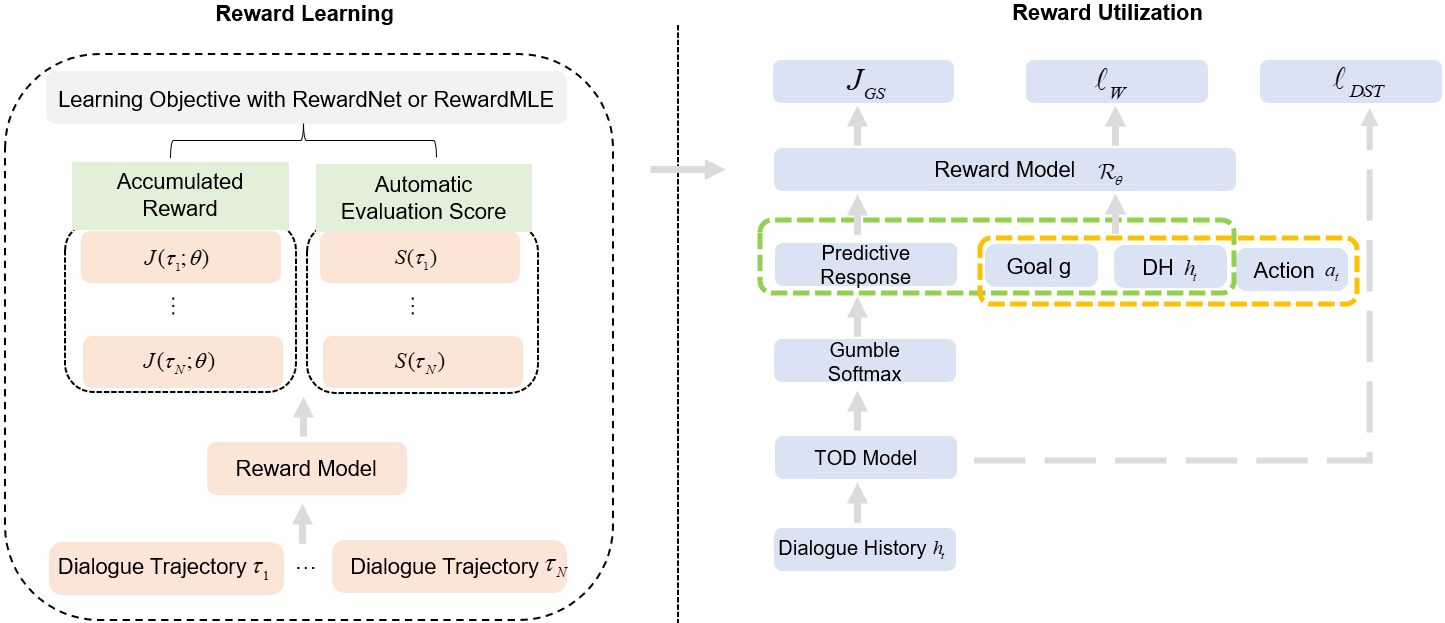
\includegraphics[width=11.5cm]{Tex/fig/Dialogue_flow.PNG}
% \vspace{-1mm}
\captionsetup{font=small}
\caption{Overview of the proposed method. 
% Some notations are labeled along with corresponding components. 
We denote ``Accumulated Reward'' for the learned accumulated reward, 
% ``Automatic Evaluation Score" for the automatic evaluation score of trajectory, 
$J(\cdot;\theta)$ for the accumulated reward of each trajectory, $S(\cdot)$ for the combined score of each trajectory,
% ``DT" the dialogue trajectory.
$\ell_\mathrm{W}$ for the weighted regularization, $\ell_{\mathrm{DST}}$ for the DST loss, 
and ``DH" for the dialogue history.
In the right panel, $(h_t, a_t, g)\sim \hat{\mathsf{D}}$.
We use BART 
% \citep{bart2019} 
for both the reward model and the ToD model.
}
\vspace{-1.5em}
\label{fig:pipeline}
\end{figure}


\myparagraph{Remark}
Eq.~\eqref{eq:final_loss} for the learning of the dialogue agent $\pi_{\phi}$ is essentially a generalized objective from several previous works.
Specifically, if we set $\alpha = 0$ and set the reward function to be constant $\gR_{\theta}(o_t, a_t, g)\equiv 1$, 
 Eq.~\eqref{eq:final_loss} reduces to the objective in MinTL, without any guidance for response-generation from the learned reward function $\gR_{\theta}$.
If we set $\alpha = 0$, and use the \rewardnet loss with $N=2$ and $\Phi=(\cdot)^{1}$ (\ie, the identity function) to train the reward function,  Eq.~\eqref{eq:final_loss} reduces to the objective in CASPI \citep{caspi2021}. 
In \Secref{sec:exp}, we demonstrate the advantages of our  techniques proposed in this section, including the \rewardnet and \rewardmle losses for reward learning, and  the $J_{\mathrm{GS}}(\pi_{\phi})$ for agent training.

% \yy{todo: add some followed up description of behavior policy and data collection}
%\yy{todo: add when we reduce to mintl, and also discussion with caspi.} \st{May be put this on Appendix? Otherwise people may be confused on how we collect the trajectories for reward learning.}

% \yy{todo: need to add some intuition and why we want to use these two loss over pairwise ones}
% \st{I have added some in the paragraph after the heading of Section 3.1}








